\documentclass[12pt]{article}
\usepackage[utf8]{inputenc}
\usepackage{graphicx}
\usepackage{framed, color}

\definecolor{shadecolor}{rgb}{0.83,1,0.8}
\begin{document}

\begin{titlepage}

\newcommand{\HRule}{\rule{\linewidth}{0.5mm}} % Defines a new command for the horizontal lines, change thickness here

\center % Center everything on the page
 
%----------------------------------------------------------------------------------------
%	HEADING SECTIONS
%----------------------------------------------------------------------------------------

\textsc{\LARGE Universidad de Concepción}\\[1.5cm] % Name of your university/college
\textsc{\Large Departamento de Ingeniería Civil Informática y Ciencias de la Computación}\\[0.5cm] % Major heading such as course name
\textsc{\large Ingeniería de Software I}\\[0.5cm] % Minor heading such as course title

%----------------------------------------------------------------------------------------
%	TITLE SECTION
%----------------------------------------------------------------------------------------

\HRule \\[0.4cm]
{ \huge \bfseries Aplicación Movil en Apoyo al Turismo en la Provincia de Arauco }\\[0.4cm] % Title of your document
\HRule \\[1.5cm]
 
%----------------------------------------------------------------------------------------
%	AUTHOR SECTION
%----------------------------------------------------------------------------------------

\begin{minipage}{0.4\textwidth}
\begin{flushleft} \large
\emph{Author:}\\
Cristobal \textsc{Donoso}
Matías \textsc{Medina}
Diego \textsc{Rodriguez}
\end{flushleft}
\end{minipage}
~
\begin{minipage}{0.4\textwidth}
\begin{flushright} \large
\emph{Supervisor:} \\
Gonzalo \textsc{Rojas} % Supervisor's Name
\end{flushright}
\end{minipage}\\[4cm]

{\large \today}\\[3cm] % Date, change the \today to a set date if you want to be precise
\vfill % Fill the rest of the page with whitespace
\end{titlepage}

%----------------------------------------------------------------------------------------
%	INTRODUCTION
%----------------------------------------------------------------------------------------
\section{Introducción}
Chile, por su geografía y diversidad climática, posee muchos lugares turísticos que yacen en el ojo de los que viajan. Sin embargo, actualmente existen lugares a pocos kilómetros de la ciudad, accesibles pero alejados en popularidad, como lo es la provincia de Arauco. Hemos escogido esta provincia dado que posee un valor cualitativo importante en el área del turismo (considerándola como una de las mayores fuentes de ingreso para la provincia) ocasionando un trade-off con el creciente avance de la gran industria.\\\\En este proyecto realizaremos un prototipo de solución el cual consiste en la creación de una aplicación móvil que ayude en la difusión, orientación y elección de puntos de interés para el turista. Se espera que esta aplicación pueda entregar un apoyo real hacia las pequeñas empresas que se encuentran registradas en el SERNATUR.\\\\Nuestra dinámica de trabajo funda sus bases en el \textbf{modelo de procesos tipo cascada} que, entre otras cosas, se caracteriza por separar las distintas fases de especificación e implementación de manera secuencial y sin retorno. Los procesos involucrados se relacionan con:
\begin{enumerate}
\item \textbf{Requerimientos:} Requisitos que debe tener el Software definidos según las necesidades de la Provincia de Arauco.
\item \textbf{Diseño del Software:} 
\item \textbf{Implementación y Testeo:}
\item \textbf{Integración:}
\item \textbf{Operación y Mantenimiento:} 
\end{enumerate}  
\newpage
\section{Disciplinas de RUP para la iteración}
\subsection{Modelado del Negocio}
\subsection{Requerimientos}
\subsection{Análisis y Diseño	} 

\begin{center}\begin{figure}[htp]
\centering
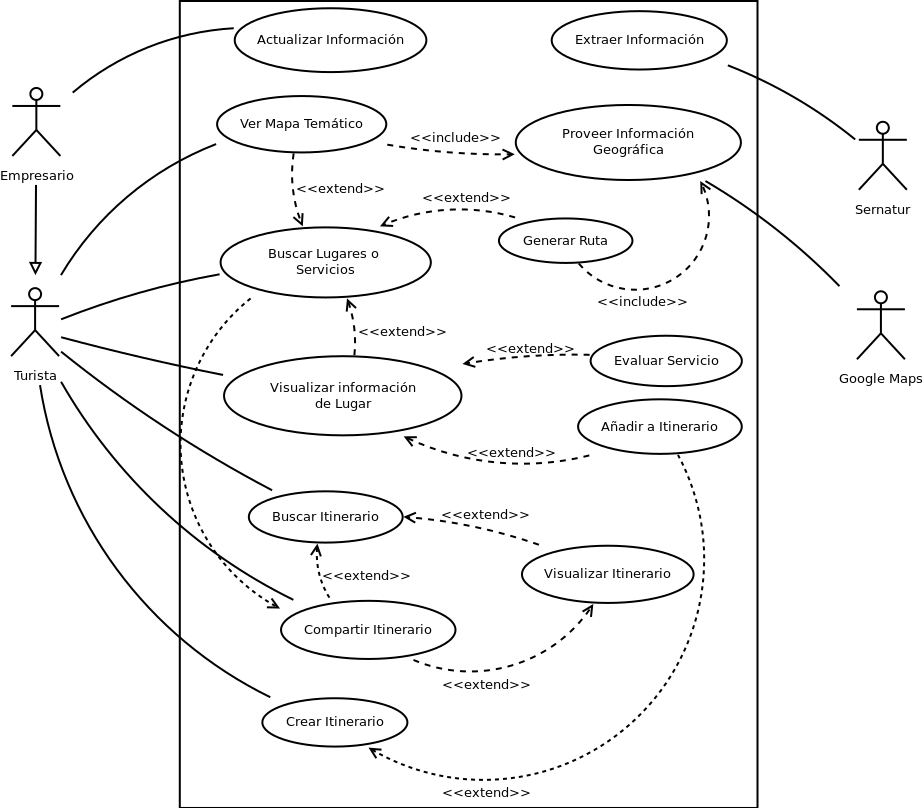
\includegraphics[scale=0.4]{Diagrama1.png}
\caption{Diagrama de Casos de Uso}
\label{}
\end{figure} \end{center} 
\newpage
\subsection{Documentación Casos de Uso}
%caso de uso ver mapa tematico
\underline{Caso de Uso:} Ver mapa temático\\\\\underline{Actor Principal}: Turista\\\\\underline{Personal involucrado e intereses}\\Turista: Quiere visualizar mapa de servicios de la provincia de Arauco.\\
Maps: Quiere recibir peticiones de PoI para mostrar en mapa de forma correcta.\\\\\underline{Precondiciones:} El sistema asigna a cada servicio un símbolo PoI.
Maps se encuentra conectado al sistema principal.\\\\\underline{Postcondiciones}: El turista visualiza un mapa ( geográfico) con marcas dónde aparecen el o los servicios que fueron seleccionados.\\\\\underline{Escenario principal de éxito:}
\begin{enumerate}
\item Se envía petición a Maps para proveer el mapa geográfico de la provincia de Arauco.
\item El turista visualiza el mapa geográfico de la provincia de Arauco.
\item El turista selecciona el o los servicios que desea visualizar en el mapa temático.
\item Se envía la petición a Maps para que provea el o los servicios (PoI) ubicados geográficamente.
\item Los servicios aparecen en el mapa geográfico según la símbolos PoI predefinidos.
\end{enumerate}
\underline{Extensiones:}
\begin{itemize}
\item1’. Falla la conexión con Maps , se muestra una alerta.
\item4’.  Falla la conexión con Maps , se muestra una alerta  y vuelve al paso 1.
\end{itemize}
%caso de uso proveer informacion geografica
\underline{Caso de Uso:}Proveer Información Geográfica \\\\\underline{Actor Principal}: Maps\\\\\underline{Personal involucrado e intereses}\\Maps: Quiere recibir peticiones de información geográfica para enviar.\\\\\underline{Precondiciones:} Maps se encuentra conectado al sistema principal.\\\\\underline{Postcondiciones}: Maps entrega la información geográfica (mapa o POI).\\\\\underline{Escenario principal de éxito:}
\begin{enumerate}
\item Maps recibe petición para mostrar un mapa geográfico o puntos de interés.
\item Maps entrega mapa geográfico o puntos de interés.
\end{enumerate}
\underline{Extensiones:}
\begin{itemize}
\item1’. Falla la conexión con Maps , se muestra una alerta.

\subsection{Implementación}
\subsection{Testing}
\subsection{Transición}
%%Conclusiones------------------
\section{Conclusiones}
\end{itemize}






























\end{document}